\documentclass[12pt]{article}
\usepackage{geometry}
\geometry{
	left=20mm,
	top=20mm,
}
\usepackage[utf8]{inputenc}
\usepackage[shortlabels]{enumitem}
\usepackage{array}
\newcolumntype{C}[1]{>{\centering\let\newline\\\arraybackslash\hspace{0pt}}m{#1}}
\usepackage[spanish,es-nodecimaldot]{babel}
 \usepackage{url}
\usepackage[spanish, fixlanguage]{babelbib}
\bibliographystyle{IEEEtran}
\usepackage{graphicx}
\graphicspath{ {./images/} }
\usepackage{amssymb}
\usepackage{amsmath}
\usepackage{subcaption}
\usepackage[linesnumbered]{algorithm2e}
\newcommand\mycommfont[1]{\footnotesize\ttfamily\textcolor{blue}{#1}}
\SetCommentSty{mycommfont}
\usepackage{tikz}
\usetikzlibrary{positioning, fit}
\usetikzlibrary{babel}
\usepackage{titlesec}
\titlespacing*{\section}
{0pt}{5.5ex plus 1ex minus .2ex}{.3ex plus .1ex}
\titlespacing*{\subsection}
{0pt}{5.5ex plus 1ex minus .2ex}{2.3ex plus .1ex}
\title{Tarea 7}

\author{
	Saul Ivan Rivas Vega \\
	\\
	Diseño y análisis de algoritmos\\
\\
	Equipo Completo:\\
		Yadira Fleitas Toranzo\\
		Diego de Jesús Isla Lopez\\
		Saul Ivan Rivas Vega\\
}

\date{\today}

\begin{document}
	\maketitle
	\pagebreak
	\section{Ejercicio 1.}
	  \paragraph{} Sea $A[1,...,n]$ un arreglo con enteros tanto positivos como negativos en sus entradas. La \textit{suma de un subarreglo} $A[i,...,j]$ es la suma de sus entradas: $\sum_{k=i}^{j}A[k]$. El problema del \textit{subarreglo de suma máxima} consiste en recibir $A$ como entrada y devolver el subarreglo de $A$ cuya suma sea la máxima posible de entre todos los subarreglos de $A$.
	  \\
	  Haz lo siguiente:
	  \\
	 \subsection{a) Diseña un algoritmo tipo \textit{divide y vencerás} que solucione el problema. Demuestra la corrección de tu algoritmo y haz un análisis de tiempo y espacio.} 
	 \subsubsection{Algoritmo} 
	 \begin{algorithm}[H]
	 	\KwData{Arreglo $A$, los índices s y t con valores s=1, y t=n.}
	 	\KwResult{Tupla $(max\_sum, i, j)$ Que representa el valor de la suma máxima y los índices $i,j$ del subarreglo $A[i,...,j]$ con dicha suma máxima.}
	 	\SetAlgoLined
	 	\tcc{Evaluamos el caso base.}
	 	\If{s = t}{
	 		return (A[s], s, t)\;
 		}
	 	
	 	\tcc{Tomamos el valor medio en el rango actual.} 
	 	mid=(s+t)/2\;
	 	\tcc{Obtener la respuesta para el rango izquierdo.}
	 	($suma_{izq}, i_{izq}, j_{izq}$) = MAXSUM(A, s, mid)\;
		\tcc{Obtener la respuesta para el rango derecho.}
		($suma_{der}, i_{der}, j_{der}$) = MAXSUM(A, mid + 1, t)\;	 
	 	\tcc{Obtener la respuesta para el rango que pasa por la mitad $mid$.}
	 	($suma_{mid}, i_{mid}, j_{mid}$) = MIDSUM(A, s, mid, t)\;
	 	
	 	return las respuestas máximas de entre las tres\;
	 	\caption{Algoritmo MAXSUM.}
	 \end{algorithm}
 \begin{algorithm}[H]
 	\KwData{Arreglo $A$, los índices s, $mid$ y t.}
 	\KwResult{Tupla $(max\_sum, i, j)$ Que representa el valor de la suma máxima y los índices $i,j$ del subarreglo $A[i,...,j]$ con dicha suma máxima con $s \leq i,j \leq t$ y además $i \leq mid \leq j$.}
 	\SetAlgoLined
 	\tcc{Inicializamos variable de la suma a la izquierda de $mid$ y el índice.}
 	$max\_suma_{izq} = -\infty$\;
 	$indice_{izq} = 0$\;
 	\tcc{Recorremos desde $mid$ hasta $s$ reduciendo $i$ en uno en cada iteración.}
 	$suma = 0$\;
 	\For{i = mid, i $\geq$ s}{
 		$suma += A[i]$\;
 		\If{$suma > max\_suma_{izq}$}{
 			$max\_suma_{izq} = suma$\;
 			$indice_{izq} = i$\;
 		}
 	}
 	\tcc{Inicializamos variable de la suma a la derecha de $mid$ y el índice.}
 	$max\_suma_{der} = -\infty$\;
 	$indice_{der} = 0$\;
 	\tcc{Recorremos desde $mid+1$ hasta $t$ incrementando $i$ en uno en cada iteración.}
 	$suma = 0$\;
 	\For{i = mid+1, i $\leq$ t}{
 		$suma += A[i]$\;
 		\If{$suma > max\_suma_{der}$}{
 			$max\_suma_{der} = suma$\;
 			$indice_{der} = i$\;
 		}
 	}
 	return ($max\_suma_{izq}+max\_suma_{der}, indice_{izq}, indice_{der}$)\;
 	\caption{Algoritmo MIDSUM.}
 \end{algorithm}
\pagebreak
\subsubsection{Correctitud.}	
\paragraph{El algoritmo MIDSUM termina.} Los dos ciclos en el algoritmo son finitos y terminan al recorrer los elementos de ($s$, $mid$) y los elementos en ($mid + 1$, $t$), es decir los elementos en el rango ($s$, $t$). Siendo $n$ la cantidad máxima de elementos en un rango $s$ y $t$, podemos decir que a lo más hará $n$ iteraciones y como en cada iteración hacemos operaciones constantes el algoritmo termina en $n$ pasos.
\paragraph{El algoritmo MAXSUM termina.} En cada invocación adicional en la ejecución del algoritmo se reduce el rango de búsqueda. En este caso el rango ($s$, $t$), se divide por la mitad en ($s$, $mid$) y ($mid + 1$, $t$). El rango no puede dividirse mas que $log_2(t-s + 1)$, que es a su vez igual a $log_2(n)$, pues es la cantidad de elementos en $A$. Así llegamos a que se realizaran $log_2(n)$ invocaciones. Y en cada invocación se realizan operaciones constantes y además se llama el algoritmo MIDSUM, el cual en el parrafo anterior vimos que termina en $n$ pasos, por lo tanto el algoritmo MAXSUM termina en $log_2(n)\times n$ pasos. 
\paragraph{El algoritmo MIDSUM devuelve el subarreglo de suma máxima tal que incluye el elemento en $mid$ en el rango $(s, t).$} El algoritmo empieza directamente con $mid$ siendo mayor siempre en un caso práctico $-\infty$ se tomará al menos ese elemento. En cada paso del primer loop lo que hace es checar la suma del subarreglo que termina en $mid$ y empieza en algún índice en el rango $(s, mid)$, pues de hecho revisa cada posición en ese rango llevando la suma acumulada y actualizando el mayor. De igual forma en el segundo loop se revisa las posibles posiciones finales del subarreglo. Como revisamos todos los posibles inicios y finales para el subarreglo y nos quedamos con los mayores respectivamente, la suma de ambos será la mayor. Así llegamos a que el la suma y los indices que devuelve MIDSUM corresponden al subarreglo de suma máxima que incluye al elemento $mid$ en el rango $(s, t)$.
\paragraph{El algoritmo MAXSUM devuelve el subarreglo de suma máxima de $A$ en el rango $(s, t).$} 
Por inducción.\\
\textbf{Invariante:} El subarreglo de suma máxima se encuentra en alguno de los 3 siguientes casos:
\begin{itemize}
	\item Esta completamente en la parte a la izquierda de $mid$.
	\item Esta completamente en la parte a la derecha de $mid$.
	\item Esta cruzando por $mid$.
\end{itemize}
Los cuales son revisados en MAXSUM partiendo en las invocaciones a la izquierda y derecha de $mid$, así como el subarreglo cruzando por $mid$ con MIDSUM.\\
\textbf{Caso base:} $s$ es igual a $t$, así mismo $mid=s$, por lo tanto el único rango es de $(s,t)$, que es igual a $(s, s)$ y a su vez $(mid, mid)$, lo cual cae en el caso 3 de la invariante.\\
\textbf{Hipótesis inductiva:} El algoritmo devolverá el subarreglo de suma máxima que se encuentre en alguno de los 3 casos mencionados.\\
Suponemos cierto para una i-ésima invocación del algoritmo. Esto implica que ya tenemos la respuesta para cuando buscamos en el rango $(s, mid)$, así como el rango $(mid + 1, t)$, los cuales corresponden a los primeros dos casos. Para el tercero y último caso debemos considerar los rangos que contienen al elemento en $mid$ y como vimos anteriormente el algoritmo MIDSUM nos devolverá el mayor. Entonces como revisamos esos tres casos y devolvemos el mayor podemos decir finalmente que el mayor rango que se encuentre en los únicos 3 casos mencionados, será revisado por el algoritmo y devuelto como respuesta.
\subsubsection{Complejidad en Tiempo.}
\paragraph{MIDSUM es de complejidad $O(n)$.} Como vimos en la sección anterior el algoritmo de MIDSUM termina después de $n$ iteraciones a lo más, por que solo recorre dos ciclos cuyo tamaño total es $n$.
\paragraph{MAXSUM es de complejidad $O(nlog(n))$.} Como vimos en la sección anterior el algoritmo de MAXSUM termina después de $nlogn$ operaciones, que es de realizar $logn$ invocaciones con a lo más $n$ operaciones en cada una por la llamada a MIDSUM, por lo que la complejidad total es $O(nlog(n))$.
Con una relación de recurrencia podemos ver la complejidad como:
\begin{figure}[h]
	\begin{center}
		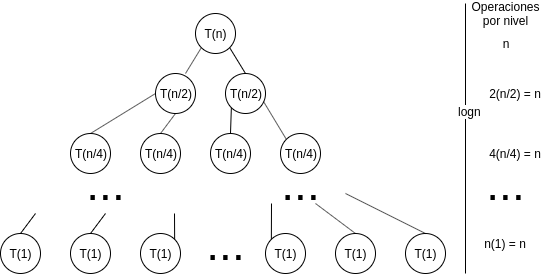
\includegraphics[scale=0.8]{recurrencia}
	\end{center}
	\caption{Recurrencia.}
\end{figure}

\begin{equation}
\begin{split}
T(n) & = 2T(n/2) + n \\
	& = 4T(n/4) + 2(n/2) + n \\
	& = 8T(n/8) + 4(n/4) + n + n \\
	\text{se pueden tener a lo mas $log_2n$ niveles en la recurrencia}... & \\
	& = T(1) + n + ... + n + n \\
	& = 1 + n + ... + n + n \\
	& = 1 + n(log_2n) \\
\end{split}
\end{equation}
\subsubsection{Complejidad en Espacio.}
\paragraph{El algoritmo MIDSUM ocupa memoria adicional de O(1).} En MIDSUM solo se inicializan de manera adicional a las entradas las variables para las sumas e índices, lo cual es de orden $O(1)$.
\paragraph{El algoritmo MAXSUM ocupa memoria adicional de $O(log_2n)$.} En cada invocación solo usamos variables adicionales de $O(1)$, sin embargo la pila de llamadas recursivas también ocupa memoria adicional, esta es equivalente a la profundidad de las invocaciones y como vimos en la sección anterior esta es de $log_2n$, por lo que ademas de las variables de $O(1)$ utilizamos $O(log_2n)$ de la pila de llamadas recursivas. Finalmente como el factor dominante es $O(log_2n)$ decimos que en espacio MAXSUM es de orden $O(log_2n)$.
\subsection{b) Diseña un algoritmo tipo \textit{programación dinámica} que solucione el problema. Demuestra la corrección de tu algoritmo y haz un análisis de tiempo y espacio.}
\subsubsection{Algoritmo}
Tomemos la siguiente función para la definición del algoritmo de programación dinámica.
\begin{equation}\label{f_ej3.2}
OPT(i) = 
\begin{cases}
\text{A[i],} &\text{i es 0}\\
\text{max(A[i], OPT(i-1) + A[i]),} &\text{en otro caso} \\
\end{cases}
\end{equation}
La ecuación \ref{f_ej3.2} representa una función que devuelve el valor de la suma máxima para un subarreglo contiguo que termina en el elemento $i$.\\
Esto es por que en cada $i$ se compara el valor de solo tomar ese elemento, o continuar con el subarreglo en el que se encuentra el elemento anterior.\\\\
\begin{algorithm}[H]\footnotesize
	\KwData{Arreglo $A$.}
	\KwResult{Tupla $(max\_sum, i, j)$ Que representa el valor de la suma máxima y los índices $i,j$ del subarreglo $A[i,...,j]$.}
	\SetAlgoLined
	\tcc{Inicializamos el arreglo para recordar respuestas anteriores de tamaño igual a $n$, es decir el tamaño del arreglo $A$.}
	$M=[n]$\;
	\tcc{Inicilizamos el valor de $M[0]$ pues solo tiene una opción, así como la suma mayor vista y el indice final del subarreglo con mayor suma.}
	$M[0] = A[0]$\;
	$suma\_mayor=A[0]$\;
	$indice\_final\_mayor=0$\;
	\tcc{Recorremos las demás posiciones desde 1 hasta $n-1$ y nos quedamos con el mayor para la respuesta.}
	\For{i = 1, i $\leq$ $n-1$}{
		$M[i]=max(A[i], A[i] + M[i-1])$\;
		\If{$M[i]>suma\_mayor$}{
			$suma\_mayor = M[i]$\;
			$indice\_final\_mayor = i$\;
		}
	}
	\tcc{Inicializamos el indice de inicio que encontraremos al reconstruir la respuesta.}
	$indice\_inicio\_mayor=0$\;
	\tcc{Reconstruimos la respuesta a partir del indice con la mayor suma, que se detiene cuando la respuesta en la posición $i$, es decir $M[i]$, haya sido solo tomar el elemento en dicha posición.}
	\For{i = $indice\_final\_mayor$, i $\geq$ $0$}{
		\If{$M[i]=A[i]$}{
			$indice\_inicio\_mayor=i$\;
			break\;
		}
	}
	return ($suma\_mayor, indice\_inicio\_mayor, indice\_final\_mayor$)\;
	\caption{Algoritmo MAXSUMDP.}
\end{algorithm}
\subsubsection{Correctitud.}
\paragraph{El algoritmo termina.} El algoritmo termina por que las únicas operaciones que se están realizando son de comparación y asignación que podemos considerar como constantes y 2 ciclos que recorren a lo más todas las $n$ posiciones en el arreglo, realizando a lo más $n$ iteraciones. Finalmente decimos que el algoritmo termina después de $2n$ iteraciones en total de los 2 ciclos.
\paragraph{El algoritmo Devuelve el subarreglo de suma máxima en $A$.} 
\paragraph{Demostremos que la función para encontrar el subarreglo de suma máxima que termina en $i$ es correcta.}
Por inducción.\\
\textbf{Invariante:} Para cada $i$ el subarreglo de suma máxima que termina en $i$ es aquel que solo contempla al elemento $A[i]$ y el subarreglo de suma máxima que termina en $i-1$ sumándole $A[i]$. \\
\textbf{Caso base:} Para $i=0$, en este caso solo queda tomar el elemento $A[0]$ cumpliendo con la invariante.\\
\textbf{Hipótesis inductiva:} Para cada $i$ solo es necesario considerar el elemento $A[i]$ y el máximo de la posición $i-1$. Esto es cierto debido a que la respuesta requiere dar un subarreglo contiguo y como en la función para la programación dinámica estamos revisando los subarreglos que terminan en cada posición $i$, necesariamente la respuesta en $i$ incluye al elemento $A[i]$.\\
Le sigue que entonces para considerar al elemento $A[i]$ como parte de un subarreglo contiguo  durante la $i$-ésima iteración, solo puede ser un subarreglo que contenga a $A[i-1]$, pues estamos considerando los subarreglos que terminan en la posición $i$.\\ Ahora entonces hay que tomar el subarreglo de mayor suma que contenga al elemento $A[i-1]$ durante la $i$-ésima iteración, sin embargo esta respuesta ya esta calculada y almacenada en $M[i-1]$.\\ Por lo tanto solo debemos tomar el máximo entre $A[i]$ y $M[i-1]+A[i]$.
\paragraph{Demostremos que el algoritmo devuelve el subarreglo contiguo de suma máxima.}
Por contradicción.\\
Supongamos que existe un subarreglo contiguo de suma máxima, cuya suma es mayor al que devolvió el algoritmo. Eso quiere decir que el algoritmo no consideró ese subarreglo de suma máxima durante la ejecución, puesto que siempre actualiza su suma máxima si encuentra una suma mayor, como se muestra en la linea $7$. Dicho subarreglo de suma máxima forzosamente tiene un índice final dentro de $A$, es decir el subarreglo de suma máxima $A[i,...,j]$ tiene a $j$ en el rango $0\leq j < n$. Sin embargo el algoritmo, en el primer ciclo, revisa la respuesta de la programación dinámica de los subarreglos que terminan en cada posición $0\leq i < n$, y por la demostración anterior, estas respuestas corresponden a los subarreglos de suma máxima que terminan en $i$. Finalmente esto es una contradicción puesto que si revisamos todos los subarreglos que terminan en una posición $0\leq j < n$ y por lo tanto no puede haber otro subarreglo contiguo de suma máxima, cuya suma sea mayor al que devolvió el algoritmo.\\
\subsubsection{Complejidad en Tiempo.}
El algoritmo como vimos termina después de $n$ iteraciones de los 2 ciclos que no están anidados y como en cada iteración se realizan asignaciones y comparaciones que podemos considerar de tiempo constante, podemos decir que se realizan $2n$ operaciones, lo cual hace que el algoritmo sea $O(2n)$ y finalmente $O(n)$.
 \subsubsection{Complejidad en Espacio.}
 El algoritmo utiliza unas variables para la suma e indice mayores, los cuales podemos considerar de $O(1)$, sin embargo utilizamos un arreglo de tamaño $n$ para almacenar las respuestas y poder reconstruir la respuesta final, por lo tanto la complejidad en memoria es de $O(n)$.
\subsection{c) Haz una comparación de tus dos algoritmos, explicando sus ventajas y desventajas del uno con respecto al otro.}
El algoritmo de divide y vencerás ocupa menos memoria adicional que el algoritmo de programación dinámica ya que trabaja en rangos en el mismo arreglo para todas las invocaciones, sin embargo esto es vienen con un costo en la eficiencia temporal ya que el algoritmo de programación dinámica es $log_2n$ veces más rápido. Ahora bien también podríamos revisar otras propiedades de los algoritmos, como que en el de programación dinámica, solo podemos calcular la respuesta para la posición $i$ una vez que hayamos calculado todas las respuestas hasta $i-1$, esto es un trabajo que no se puede paralelizar, a diferencia del algoritmo de divide y vencerás, el cuál aunque de igual forma requiere que sus invocaciones terminen, estas pueden ser paralelizables puesto que trabajan con rangos disjuntos.\\
En general podemos concluir que para una aplicación mas robusta el algoritmo de divide y vencerás puede aprovechar distintas arquitecturas de implementación o impactar en el ahorro de memoria, y el algoritmo de programación dinámica si se puede hacer uso de mas memoria para acelerar significativamente la eficiencia del cálculo de la respuesta.
\section{Diseña un algoritmo que tome como entrada una gráfica dirigida G con pesos en sus aristas, w : E  $\rightarrow$ Z, y responda a lo siguiente:}
\begin{itemize}
	\item Si $G$ no tiene ciclos de pesos negativo, entonces responde FALSE.
	\item De otra forma, el algoritmo responde TRUE y además devuelve un ciclo $C$ de $G$ de peso negativo.
\end{itemize}
\subsection{Algoritmo}
\begin{algorithm}[H]
	\KwData{Gráfica dirigida $G = (V,E)$ con aristas ponderadas.}
	\KwResult{Tupla (TRUE, $conjunto\_nodos\_en\_ciclo$) si es que hay un ciclo de peso negativo, o la tupla (FALSE, $\emptyset$) en caso contrario.}
	\SetAlgoLined
	\tcc{Recorremos cada nodo y corremos el algoritmo LlegaCicloNegativo para revisar si tomando como origen a ese nodo $v$ llegamos a un ciclo negativo para devolverlo como respuesta.}
	\ForEach{$v\in V$}{
		($hay\_ciclo$, $conjunto\_nodos\_en\_ciclo$) = LlegaCicloNegativo($G$,$v$)\;
		\If{$hay\_ciclo$ = TRUE}{
			return ($TRUE, conjunto\_nodos\_en\_ciclo$)\;
		}
	}
	return (FALSE, $\emptyset$)\;
	\caption{Algoritmo GetNegativeCycle.}
\end{algorithm}
\begin{algorithm}[H]\small
	\KwData{Gráfica dirigida $G = (V,E)$ con aristas ponderadas y un nodo origen $s$.}
	\KwResult{Tupla (TRUE, $conjunto\_nodos\_en\_ciclo$) si es que hay un ciclo de peso negativo al que se llega a partir del nodo origen $s$, o la tupla (FALSE, $\emptyset$) en caso contrario.}
	\SetAlgoLined
	\tcc{Inicializamos los arreglos para correr el algoritmo de Bellman-Ford.}
	\ForEach{$v\in V$}{
		distancia[$v$] = $\infty$\;
		padre[$v$] = -1\;
	}
	\tcc{Inicializamos el valor de distancia para para el nodo origen.}
	distancia[s] = 0\;
	\tcc{Realizamos $n$ 'relajaciones', donde $n=|V|$, como en el algoritmo de Bellman-Ford, solo que realizamos $n$ en lugar de $n-1$,  si existió algún nodo que disminuyo su distancia y además era la $n$-ésima relajación, lo guardamos pues es parte de un ciclo negativo.}
	$nodo\_en\_ciclo\_negativo=-1$\;
	\For{i = 1, i $\leq$ $n$}{
		\ForEach{$(u,v, peso) \in E$}{
			\If{$distancia[u] + peso < distancia[v]$}{
				distancia[v] = distancia[u] + peso\;
				padre[v] = u\;
				\If{i = n}{
					$nodo\_en\_ciclo\_negativo=v$\;
				} 
			}
		}
	}
	\tcc{Revisamos si es que no existió dicho nodo que disminuyo su distancia en la $n$-ésima relajación.}
	\If{$nodo\_en\_ciclo\_negativo$ = -1}{
		return (FALSE, $\emptyset$)\;
	}
	\tcc{En este punto si existió dicho nodo que disminuyo su distancia en la $n$-ésima relajación.}
	\tcc{Inicializamos el conjunto respuesta.}	
	$conjunto\_nodos\_en\_ciclo = \emptyset$\;
	\tcc{Recorremos la lista de padres del nodo en el ciclo hasta llegar al mismo nodo original.}
	\ForEach{nodo $n$ en la cadena de padres de $nodo\_en\_ciclo\_negativo$ }{
		\tcc{Agregamos el nodo $n$ al conjunto respuesta.}
		$conjunto\_nodos\_en\_ciclo \leftarrow n$\;
		\If{n = $nodo\_en\_ciclo\_negativo$ And $|conjunto\_nodos\_en\_ciclo| > 1$}{
			break\;
		}
	}
	return ($TRUE, conjunto\_nodos\_en\_ciclo$)\;
	\caption{Algoritmo LlegaCicloNegativo.}
\end{algorithm}
\subsection{Explicación Correctitud}
\paragraph{El algoritmo LlegaCicloNegativo Termina.}
El algoritmo termina por que se realizan 2 ciclos for anidados, con el primer ciclo for recorriendo los valores desde 1 hasta $n$ que representan las $n - 1$ relajaciones en el algoritmo de Bellman-Ford con una relajación adicional con el propósito de encontrar el ciclo negativo. Esto da un total de $n$ relajaciones, y cada relajación recorre todas las aristas de la gráfica, siendo entonces un total de $n\times|E|$ iteraciones en total. Como en cada iteración se realizan asignaciones y comparaciones podemos considerarlas de tiempo constante. El valor máximo de $|E|$ puede llegar a ser cercano a $|V|^2$ que es el caso cuando todos los nodos tienen una arista todos los otros nodos. Y como estamos considerando a $n=|V|$, entonces el algoritmo realizaría un total de $n^3$. Adicionalmente si es que hay un ciclo negativo se realiza otro ciclo for que sigue la cadena de padres, el cual en el peor de los casos incluye a todos los nodos, siendo $n$ iteraciones más. Finalmente decimos que el algoritmo termina después de $n^3 + n$ operaciones.
\paragraph{El algoritmo GetNegativeCycle Termina.}
El algoritmo termina por que se realizan 1 solo ciclo for, el cual realiza $n$ iteraciones con $n=|V|$, y en cada iteración se llama al algoritmo LlegaCicloNegativo, el cuál anteriormente vimos que realiza $n^3$ iteraciones. Con $n$  llamadas a una función que realiza $n^3$ operaciones, finalmente decimos que el algoritmo termina después de a lo más $n^4$ operaciones.
\paragraph{El algoritmo LlegaCicloNegativo devuelve un ciclo de peso negativo en $G$ al cuál se llega a partir del nodo origen $s$}
Originalmente el algoritmo de Bellman-Ford en el que esta basado LlegaCicloNegativo, realiza $n-1$ relajaciones. Son $n-1$ iteraciones porque se toma en cuenta la propiedad de que un camino mínimo simple que conecta a un par de nodos en una gráfica conexa con $n$ nodos tiene a lo más $n-1$ aristas. La razón de esto es que tener una gráfica conexa con $n$ nodos y $n$ aristas tiene un ciclo, y a su vez considerar tomar un ciclo para mejorar la distancia a un nodo significaría que podemos recorrer ese mismo ciclo un número arbitrario de veces y seguir mejorando la distancia a ese nodo, lo cual infiere que recorrer el ciclo resta distancia y que por lo tanto es de peso negativo.\\
Al realizar $n$ iteraciones y algún nodo mejora su distancia estamos en el caso mencionado anteriormente y este nodo forma parte del ciclo negativo que mejoró su distancia en la $n$-ésima relajación.\\
Finalmente como en cada ocasión que reducimos la distancia a un nodo actualizamos el padre para ese nodo, el arreglo de $padres$ al ser recorrido tendrá los nodos en el ciclo negativo, el cual es devuelto como respuesta en caso de existir dicho nodo que mejoró su distancia en la $n$-ésima relajación.\\
\paragraph{El algoritmo GetNegativeCycle devuelve un ciclo de peso negativo en la gráfica $G$.}
En este caso por la explicación anterior podemos asumir correcto el funcionamiento del algoritmo LlegaCicloNegativo, y ahora por contradicción explicar que GetNegativeCycle es correcto. 
Supongamos que existe al menos un ciclo de peso negativo en $G$ y nuestro algoritmo no encontró ninguno. Eso quiere decir que no revisamos ni un solo nodo el cual pueda llegar al ciclo, ya que si lo hubiéramos revisado el algoritmo LlegaCicloNegativo nos lo hubiera devuelto.
Pero esto es una contradicción por que llamamos a LlegaCicloNegativo en todos los nodos $v\in V$ de la gráfica y no pudimos revisar y a la vez ignorar a algún nodo $v$ que si estuviera en el ciclo. Finalmente decimos que el algoritmo GetNegativeCycle devuelve un ciclo de peso negativo en la gráfica $G$.
\subsection{Explicación Complejidad en tiempo}
\paragraph{El algoritmo LlegaCicloNegativo es de complejidad $O(n^3)$.}
Como vimos en la explicación de que termina el algoritmo, este termina después de $n^3+n$ iteraciones y podemos considerar las operaciones de asignación y comparación como de tiempo $O(1)$. Finalmente decimos que el algoritmo es de orden $O(n^3 + n)$, que tomando el factor dominante es $O(n^3)$.
\paragraph{El algoritmo GetNegativeCycle es de complejidad $O(n^4)$.}
Como vimos en la explicación de que termina el algoritmo, este termina después de $n^4$ iteraciones y podemos considerar las operaciones de asignación y comparación como de tiempo $O(1)$. Finalmente decimos que el algoritmo es de orden $O(n^4)$.
\subsection{Explicación Complejidad en espacio}
\paragraph{El algoritmo LlegaCicloNegativo ocupa espacio $O(n)$.}
El algoritmo tiene solo como memoria adicional algunas variables para guardar el nodo en el ciclo o los indices en los ciclos for, los cuales podemos considerar $O(1)$. Sin embargo hacemos uso de un arreglo de padres y distancias para cada nodo los cuales son $O(|V|)$, lo cual es $O(n)$, de igual forma tenemos el conjunto respuesta para los nodos en el ciclo de peso negativo, el cual podría albergar a todos los nodos en $G$, por lo tanto es de $O(n)$. Finalmente tenemos que el algoritmo tiene una complejidad en espacio de orden $O(3n)$, el cual es $O(n)$.
\paragraph{El algoritmo GetNegativeCycle ocupa espacio $O(n)$.}
El algoritmo solo ocupa la variable que le devuelve el algoritmo LlegaCicloNegativo, el cual es de $O(n)$. Finalmente tenemos que es de orden $O(n)$.
\end{document}  